\section{Linguaggi Context-Free}
Abbiamo visto che esistono \textit{linguaggi non regolari} (ad esempio $\{0^n1^n | n\geq 0\}$),
Consideriamo ora una classe più grande di linguaggi, i \g{Linguaggi Context-free (CFL)},
usati nello studio dei linguaggi naturali dal 1950, e nello studio dei compilatori dal 1960.
Vedremo dunque due metodi per descrivere un linguaggio CFL:
\begin{itemize}
	\item Grammatiche Context-free
		% link automi a pila
	\item Automi a pila (pushdown automata)
\end{itemize}

\subsection{Grammatiche Context-free}
Le grammatiche context-free sono un metodo più potente per descrivere i linguaggi, 
si prestano particolarmente bene a descrivere comportamenti ricorsivi all'interno di un linguaggio. \\
Inizialmente sono state utilizzate per descrivere i \g{linguaggi naturali} 
%link grammatica per l'inglese
(vedi Una grammatica per l’inglese), 
oggi sono fondamentali per lo sviluppo dei *parser*.

Vediamo ad esempio la grammatica $G_1$:

$$A\rightarrow 0A1$$
$$A\rightarrow B$$
$$B\rightarrow \#$$
Quello che possiamo notare è la presenza di 
\begin{itemize}
	\item un insieme di \g{regole di sostituzione} (o \textit{produzioni})
	\item alcune \g{variabili} ($A$ e $B$ )
	\item i \g{terminali} ossia i simboli dell'alfabeto ($0,1,\#$)
	\item una \g{variabile iniziale} $A$ 
\end{itemize}
\begin{enumerate}
	\item Scrivi la variabile iniziale
	\item Trova una variabile che è stata scritta e una regola che inizia con quella variabile.
		Sostituisci la variabile con il lato destro della regola. 
	\item Ripeti 2. fino a quando non ci sono più variabili.
\end{enumerate}

\paragraph{Esempio per $G_1$}
$$A\Rightarrow 0A1\Rightarrow 00A11 \Rightarrow 000A111\Rightarrow 000\#111$$
La sequenza di sostituzioni si chiama \g{Derivazione di 000\#111}

\subsection{Albero sintattico}
Una derivazione definisce un \g{albero sintattico (parse tree)}\\
\begin{center}
	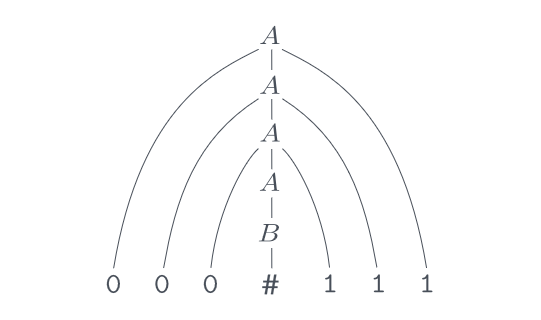
\includegraphics[scale=0.5]{img/alberosintattico.png} 
\end{center}
\begin{itemize}
	\item la radice è la variabile iniziale
	\item i nodi interni sono variabili 
	\item le foglie sono terminali 
\end{itemize}

Tutte le stringhe generate in questo modo costituiscono il *linguaggio della grammatica* $G_1$, ossia $L(G_1)$. 

\subsection{Una grammatica per l’inglese}
Definiamo $G_2$ nel seguente modo: \\
$\langle SENTENCE \rangle \rightarrow \langle NOUN$-$PHRASE\rangle \langle VERB$-$PHRASE \rangle$\\
$\langle NOUN$-$PHRASE\rangle \rightarrow \langle CMPLX$-$NOUN\rangle$\\
$\langle NOUN$-$PHRASE\rangle  \rightarrow \langle CMPLX$-$NOUN \rangle \langle PREP$-$PHRASE \rangle$ \\
$\langle VERB$-$PHRASE \rangle  \rightarrow \langle CMPLX$-$VERB \rangle$\\
$\langle VERB$-$PHRASE \rangle  \rightarrow \langle CMPLX$-$VERB \rangle \langle PREP$-$PHRASE \rangle$\\
$\langle PREP$-$PHRASE \rangle  \rightarrow \langle PREP\rangle\langle CMPLX$-$NOUN \rangle$\\
$\langle CMPLX$-$NOUN \rangle → \langle ARTICLE \rangle \langle NOUN\rangle$\\
$\langle CMPLX$-$VERB \rangle → \langle VERB\rangle | \langle VERB\rangle \langle NOUN$-$PHRASE\rangle$\\
$\langle ARTICLE \rangle \rightarrow$  \t{a | the}\\
$\langle NOUN\rangle\rightarrow$  \t{boy | girl | flower}\\
$\langle VERB\rangle\rightarrow$ \t{touches | likes | sees}\\
$\langle PREP\rangle\rightarrow$ \t{with}\\

\nin La grammatica $G_2$ ha 10 variabili ($SENTENCE$ , $NOUN$-$PHRASES$, eccetera...), 27 terminali, 
ovvero i simboli dell'alfabeto inglese standard, e 18 regole. Tra le stringe di $L(G_2)$ vi sono \\

	\t{a boy sees}
	
	\t{the boy sees a flower}
	
	\t{a girl with a flower likes the boy}\\
	\\
Ognuna di queste stringhe ha una derivazione nella grammatica $G_2$, ad esempio \\
$\langle SENTENCE \rangle \rightarrow \langle NOUN$-$PHRASE\rangle \langle VERB$-$PHRASE \rangle$

$\rightarrow\langle CMPLX$-$NOUN\rangle \langle VERB$-$PHRASE \rangle$

$\rightarrow  \langle ARTICLE \rangle \langle NOUN\rangle \langle VERB$-$PHRASE \rangle$

$\rightarrow$ \t{a} $\langle NOUN\rangle\langle VERB$-$PHRASE\rangle$

$\rightarrow$ \t{a boy} $\langle VERB$-$PHRASE\rangle$

$\rightarrow$ \t{a boy} $\langle CMPLX$-$VERB\rangle$

$\rightarrow$ \t{a boy} $\langle VERB\rangle$

$\rightarrow$ \t{a boy sees}
			

\subsection{Definizione di grammatica context-free}
Una grammatica context-free è una quadrupla $(V,\Sigma,R,S)$ dove 
\begin{itemize}
	\item $V$ è un insieme finito di \g{variabili}
	\item $\Sigma$ è un insieme finito di \g{terminali} disgiunto da $V$ 
	\item $R$ è un insieme di \g{regole}, dove ogni regola è una variabile e una stringa di variabili e terminali 
	\item $S\in V$ è la \g{variable iniziale}
\end{itemize}
Se $u, v , w$  sono stringhe di variabili e terminali e $A \rightarrow w$ è una regola:
\begin{itemize}
	\item $uAv$  \g{produce} $uwv : uAv \Rightarrow uwv$ 
	\item $u$ \g{deriva} $v : u \Rightarrow^* v$ se:
		\begin{itemize}
			\item $u = v$  , oppure
			\item esiste una sequenza $u1, u2, \dots, uk$ tale che
				$u \Rightarrow u1 \Rightarrow u2 \Rightarrow \dots \Rightarrow uk \Rightarrow v$
				$\Rightarrow$ 
		\end{itemize}
	\item il \g{linguaggio della grammatica} è $L(G) = \{w \in \Sigma^* \mid S \Rightarrow^* w \}$
\end{itemize}

\subsection{Esempi}
\subsubsection{Parentesi}
Consideriamo la grammatica $G_3 = \langle \{S\}, \{a,b\}, R, S\rangle$.  L'insieme delle regole della grammatica $G_3$ , ossia $R$, è
$$S\rightarrow aSb \mid SS \mid \varepsilon$$
Questa grammatica genera stringhe come 
\begin{itemize}
	\item \t{abab}: $S\rightarrow SS\rightarrow abS \rightarrow abab$ 
	\item \t{aaabbb} $S\rightarrow aSb\rightarrow aaSbb \rightarrow aaaSbbb\rightarrow aaabbb$ 
	\item \t{aababb}: $S\rightarrow aSb\rightarrow aSSb\rightarrow aabSb\rightarrow aababb$ \\
\end{itemize}
Si può più dedurre più facilmente di che linguaggio si tratta pensando ad \t{a} come ad una parentesi aperta "(" e a \t{b}
come ad una parentesi chiusa ")". \\
Visto in questo modo, $L(G_3)$ è il linguaggio di tutte le stringhe di \g{parentesi correttamente annidate}.\\
Si osservi che il lato destro di una regola può essere la parola vuota $\varepsilon$ 

\subsubsection{Operazioni aritmetiche}
Si consideri la grammatica $G_4 = (V,\Sigma, R, \langle EXPR \rangle)$\\
$V$ è $\{\langle EXPR \rangle, \langle TERM \rangle, \langle FACTOR \rangle\}$ e $\Sigma$ è $\{a, +, \times, (,)\}$ \\
Le regole sono: \\
	
	$\langle EXPR \rangle \rightarrow \langle EXPR \rangle + \langle  TERM\rangle \mid \langle  TERM\rangle$
	
	$\langle TERM \rangle \rightarrow \langle TERM\rangle \times \langle FACTOR\rangle \mid \langle FACTOR \rangle$ 
	
	$\langle FACTOR\rangle \rightarrow (\langle EXPR\rangle) \mid a$\\
\\
Le due stringhe \t{a+axa} e \t{(a+a)xa} possono essere generate dalla grammatica $G_4$, e questi sono i loro alberi sintattici. \\
\begin{center}
	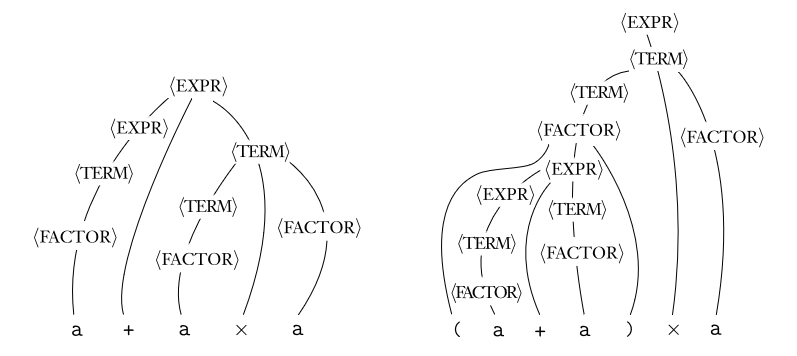
\includegraphics[scale=0.5]{img/alberi_g_4.png}
\end{center}
\subsection{Come si progetta una grammatica context-free}
Abbiamo appena visto la grammatica $G_4$. Tale grammatica potrebbe benissimo costituire una sottogrammatica
di un \textit{linguaggio di programmazione}, in quanto le operazioni aritmetiche sono una componente 
fondamentale dei linguaggi di programmazione. \\
In questo e in altri svariati contesti è probabile imbattersi in una CFG (context-free grammatic) composta da altre grammatiche meno complesse.
Per unire queste grammatiche è necessario creare una regola 
$S \rightarrow S_1 \mid S_2 \mid \dots \mid S_k$,
dove $S_1\dots S_k$ sono le variabili iniziali di ognuna delle grammatiche comprese nel linguaggio. \\
\\
Un esempio banale:
Se volessimo costruire la grammatica $\{0^n1^n\mid n\geq 0\}\cup \{1^n0^n\mid n\geq 0\}$ 
è necessario costruire la prima grammatica $$S_1\rightarrow 0S_11\mid \varepsilon$$
poi quella per la seconda $$S_2 \rightarrow 1S_20\mid\varepsilon$$
La grammatica che comprende entrambe sarà quindi l'insieme di queste tre regole:
$$ S\rightarrow S_1\mid S_2$$
$$S_1\rightarrow 0S_11\mid\varepsilon$$
$$S_2\rightarrow 1S_20\mid\varepsilon$$
Sebbene si tratti di un linguaggio non regolare è solitamente più facile costruire una grammatica per un linguaggio regolare partendo dal suo DFA.

\subsection{Forma normale di Chomsky}
\subsubsection{Ambiguità}
Una grammatica CFG può generare una stessa stringa a partire dall'applicazione di derivazioni diverse, ad esempio la grammatica $G_4$ è in grado di produrre la stringa 
\t{a + a x a}  con i seguenti alberi di derivazione:\\
\begin{center}
	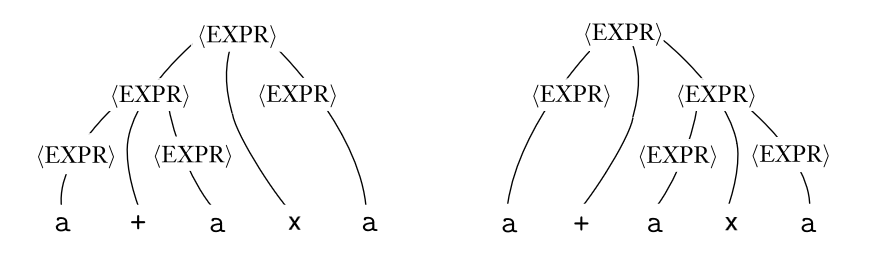
\includegraphics[scale=0.5]{img/ambiguita.png}\\
\end{center}
Questa due casi costituiscono un \g{ambiguità}.
\begin{itemize}
	\item Una stringa $w$ è derivata ambiguamente dalla grammatica $G$ se esistono due o più alberi sintattici che la generano
	\item \g{Equivalentemente}: Una stringa $w$ è derivata ambiguamente dalla grammatica $G$
		se esistono due o più derivazioni a sinistra che la generano
	\item Una grammatica è ambigua se genera almeno una stringa ambiguamente
\end{itemize}
\textit{Spesso dunque è preferibile ricavare una forma normalizzata di una CFG per poterla analizzare meglio.}\\
Una delle forme più semplici ed utili è appunto la forma normale di Chomsky. 

\subsubsection{Definizione della forma normale di Chomsky}
Una grammatica context-free è in forma normale di Chomsky se ogni regola è della forma 

$$A\rightarrow BC$$
$$A \rightarrow a$$Dove $a$ è un terminale e $B, C$ non possono essere la variabile iniziale. 
Inoltre, ci può essere la regola iniziale $S\rightarrow\varepsilon$ per la variabile iniziale $S$.

\begin{center}
	\textit{Ogni CFG è generata da una forma normale di Chomsky}\\
	di conseguenza\\
	\textit{Ogni CFG è riducibile ad una forma normale di Chomsky}
\end{center}

\subsubsection{Come passare ad una forma normale di Chomsky}
\begin{enumerate}
	\item aggiungiamo una nuova variabile iniziale
	\item eliminiamo le $\varepsilon$-regole $A \rightarrow\varepsilon$ 
	\item eliminiamo le regole unitarie $A\rightarrow B$ 
	\item trasformiamo le regole rimaste nella forma corretta
\end{enumerate}

\paragraph{Esempio}
Trasformiamo la grammatica $G_6$ in forma normale di Chomsky:
$$S\rightarrow ASA\mid aB$$
$$A\rightarrow B\mid S$$ $$B\rightarrow b\mid \varepsilon$$
\begin{enumerate}
	\item Aggiungiamo una nuova variabile iniziale $S_0\rightarrow S$ 
		\textit{Questo ci serve ad evitare che la variabile iniziale compaia a \g{destra} di una regola di derivazione}
	\item Eliminiamo le $\varepsilon$-regole $A\rightarrow\varepsilon$ 
		\begin{itemize}
			\item Se $A\rightarrow\varepsilon$ è una regola dove $A$ non è la variabile iniziale. 
			\item Per ogni regola del tipo $R\rightarrow uAv$ aggiungiamo la regola $$R\rightarrow uv$$
				\g{Attenzione}: Nel caso di più occorrenze di $A$ consideriamo tutti i casi: per le regole come 
			$R\rightarrow uvAw\mid uAvw\mid uvw$ 
			\item Nel caso di regole $R\rightarrow A$ aggiungiamo $R\rightarrow\varepsilon$ solo se non abbiamo già eliminato $R\rightarrow\varepsilon$ 
			\item ripetere fino a che non sono state eliminate tutte le $\varepsilon$-regole
		\end{itemize}

	\item  Eliminare le \g{regole unitarie} $A\rightarrow B$ :
		\begin{itemize}
			\item  Se $A\rightarrow B$ è una regola unitaria 
			\item Per ogni regola del tipo $B\rightarrow u$, aggiungiamo la regola unitaria eliminata in precedenza
			\item ripetere finché non sono state eliminate tutte le regole unitarie
		\end{itemize}
	\item Trasformiamo le regole rimaste nella forma corretta: 
		\begin{itemize}
			\item Se $A\rightarrow u_1u_2\dots u_k$ è una regola tale che 
				\begin{itemize}
					\item Ogni $u_i$ è una variabile o un terminale 
					\item $k\geq 3$ 
				\end{itemize}
			\item sostituisci la regola con la catena di regole 
	  		$A\rightarrow u_1A_1$, $A_1\rightarrow u_2A_2$, $A_@\rightarrow u_3A_3$ $\dots$ $A_{k-2}\rightarrow u_{k-1}u_k$ 
			\item  rimpiazza ogni terminale $u_i$; sul lato destro di una regola con una nuova variabile
				$U_i$ e aggiungi la regola $$U_i\rightarrow u_i$$
			\item ripetere per ogni regola non corretta
		\end{itemize}
\end{enumerate}
